\LARGE
State Beispiel
\label{subsec:state-example}
\large

Rust Code:

\begin{verbatim}
use tauri::State;
struct MyState(String);
#[tauri::command]
fn get_value(state: State<'_, MyState>) -> String {
    state.0.clone()
}
fn main() {
    tauri::Builder::default()
        .manage(MyState("Hello from backend".to_string())) // Initial value
        .invoke_handler(tauri::generate_handler![get_value])
        .run(tauri::generate_context!())
        .expect("error while running tauri application");
}
\end{verbatim}

Frontend in Typescript

\begin{verbatim}
'use client';
import { useEffect, useState } from 'react';
import { invoke } from '@tauri-apps/api/tauri';
export default function GetStateExample() {
  const [value, setValue] = useState<string>('');
  useEffect(() => {
    async function fetchValue() {
      const result = await invoke<string>('get_value');
      setValue(result);
    }
    fetchValue();
  }, []);
  return (
    <div>
      <h1>Backend State</h1>
      <p>{value}</p>
    </div>
  );
}
\end{verbatim}


\begin{figure}[htbp]
  \centering
  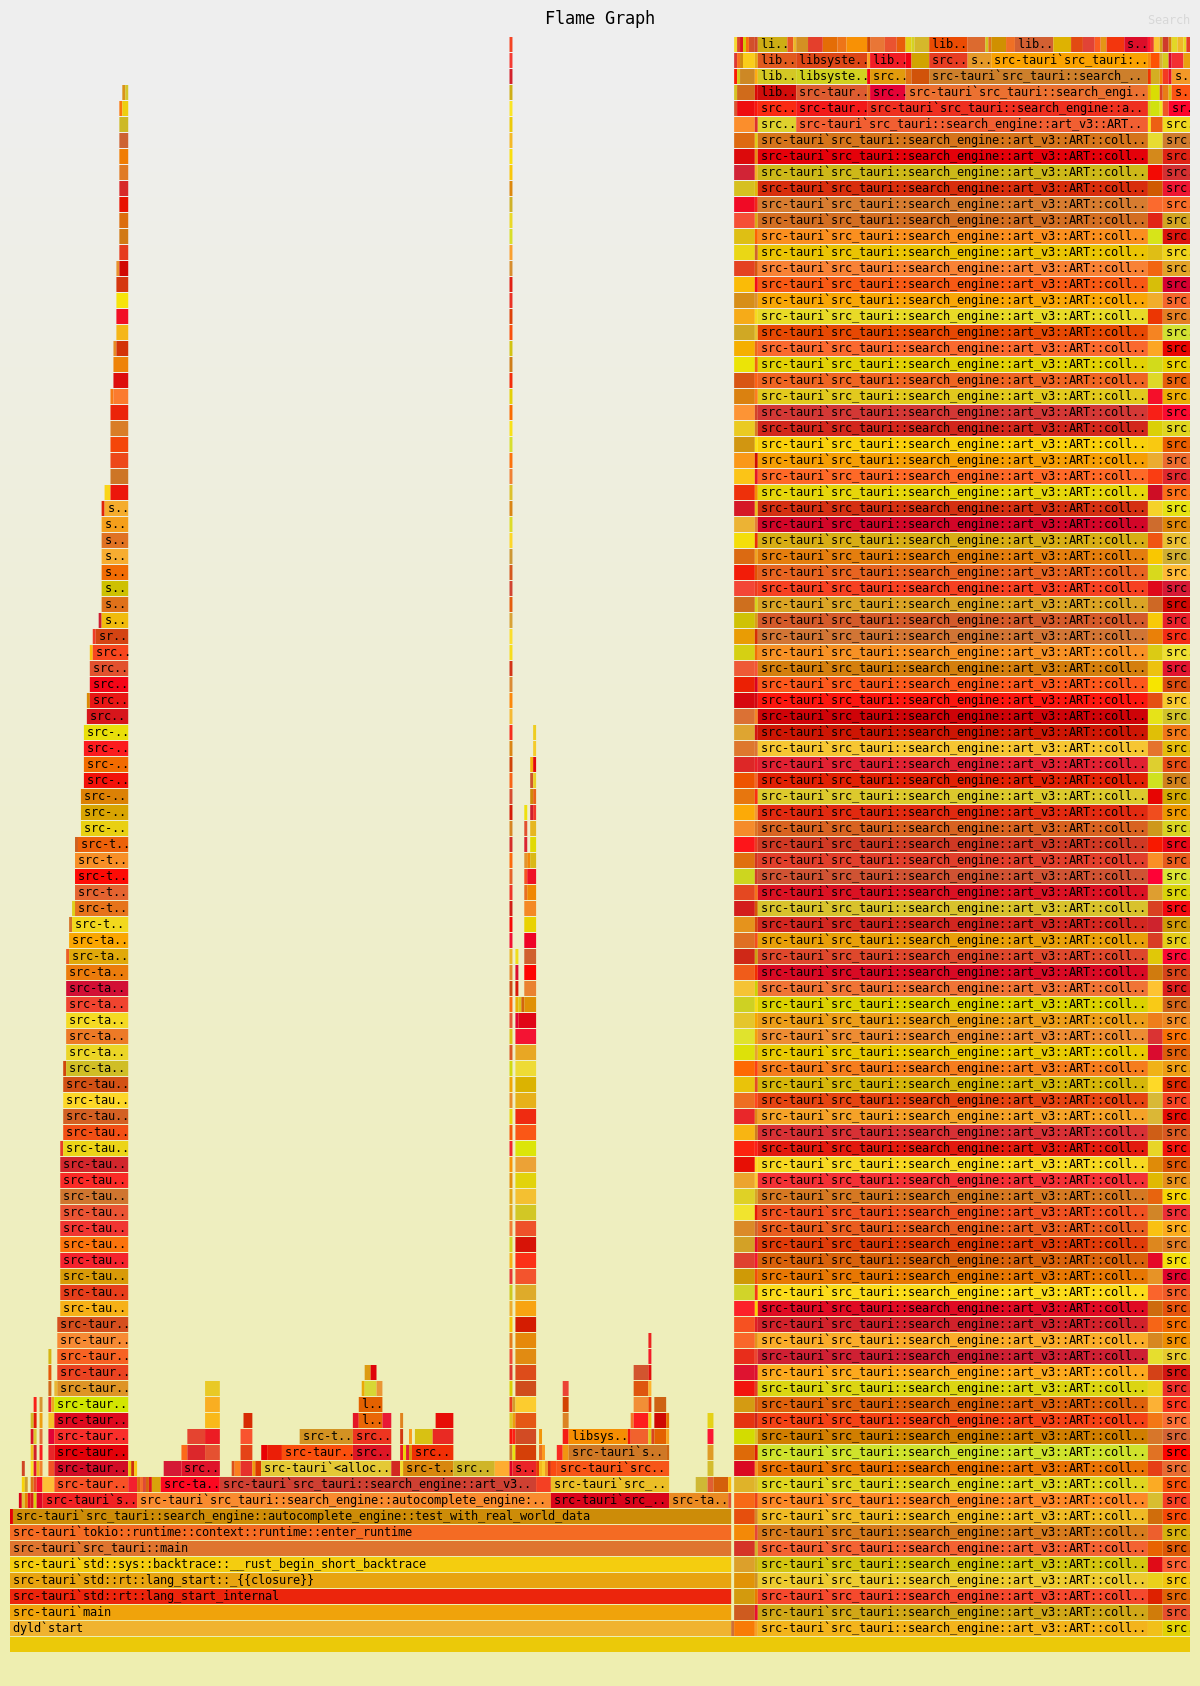
\includegraphics[width=1.0\textwidth]{./flamegraphs/test_with_real_world_data_500.png}
  \caption{Flamegraph von einem Searchengine Durchlauf mit 500 Einträgen}
  \label{fig:first_flame_graph}
\end{figure}

\begin{figure}[htbp]
  \centering
  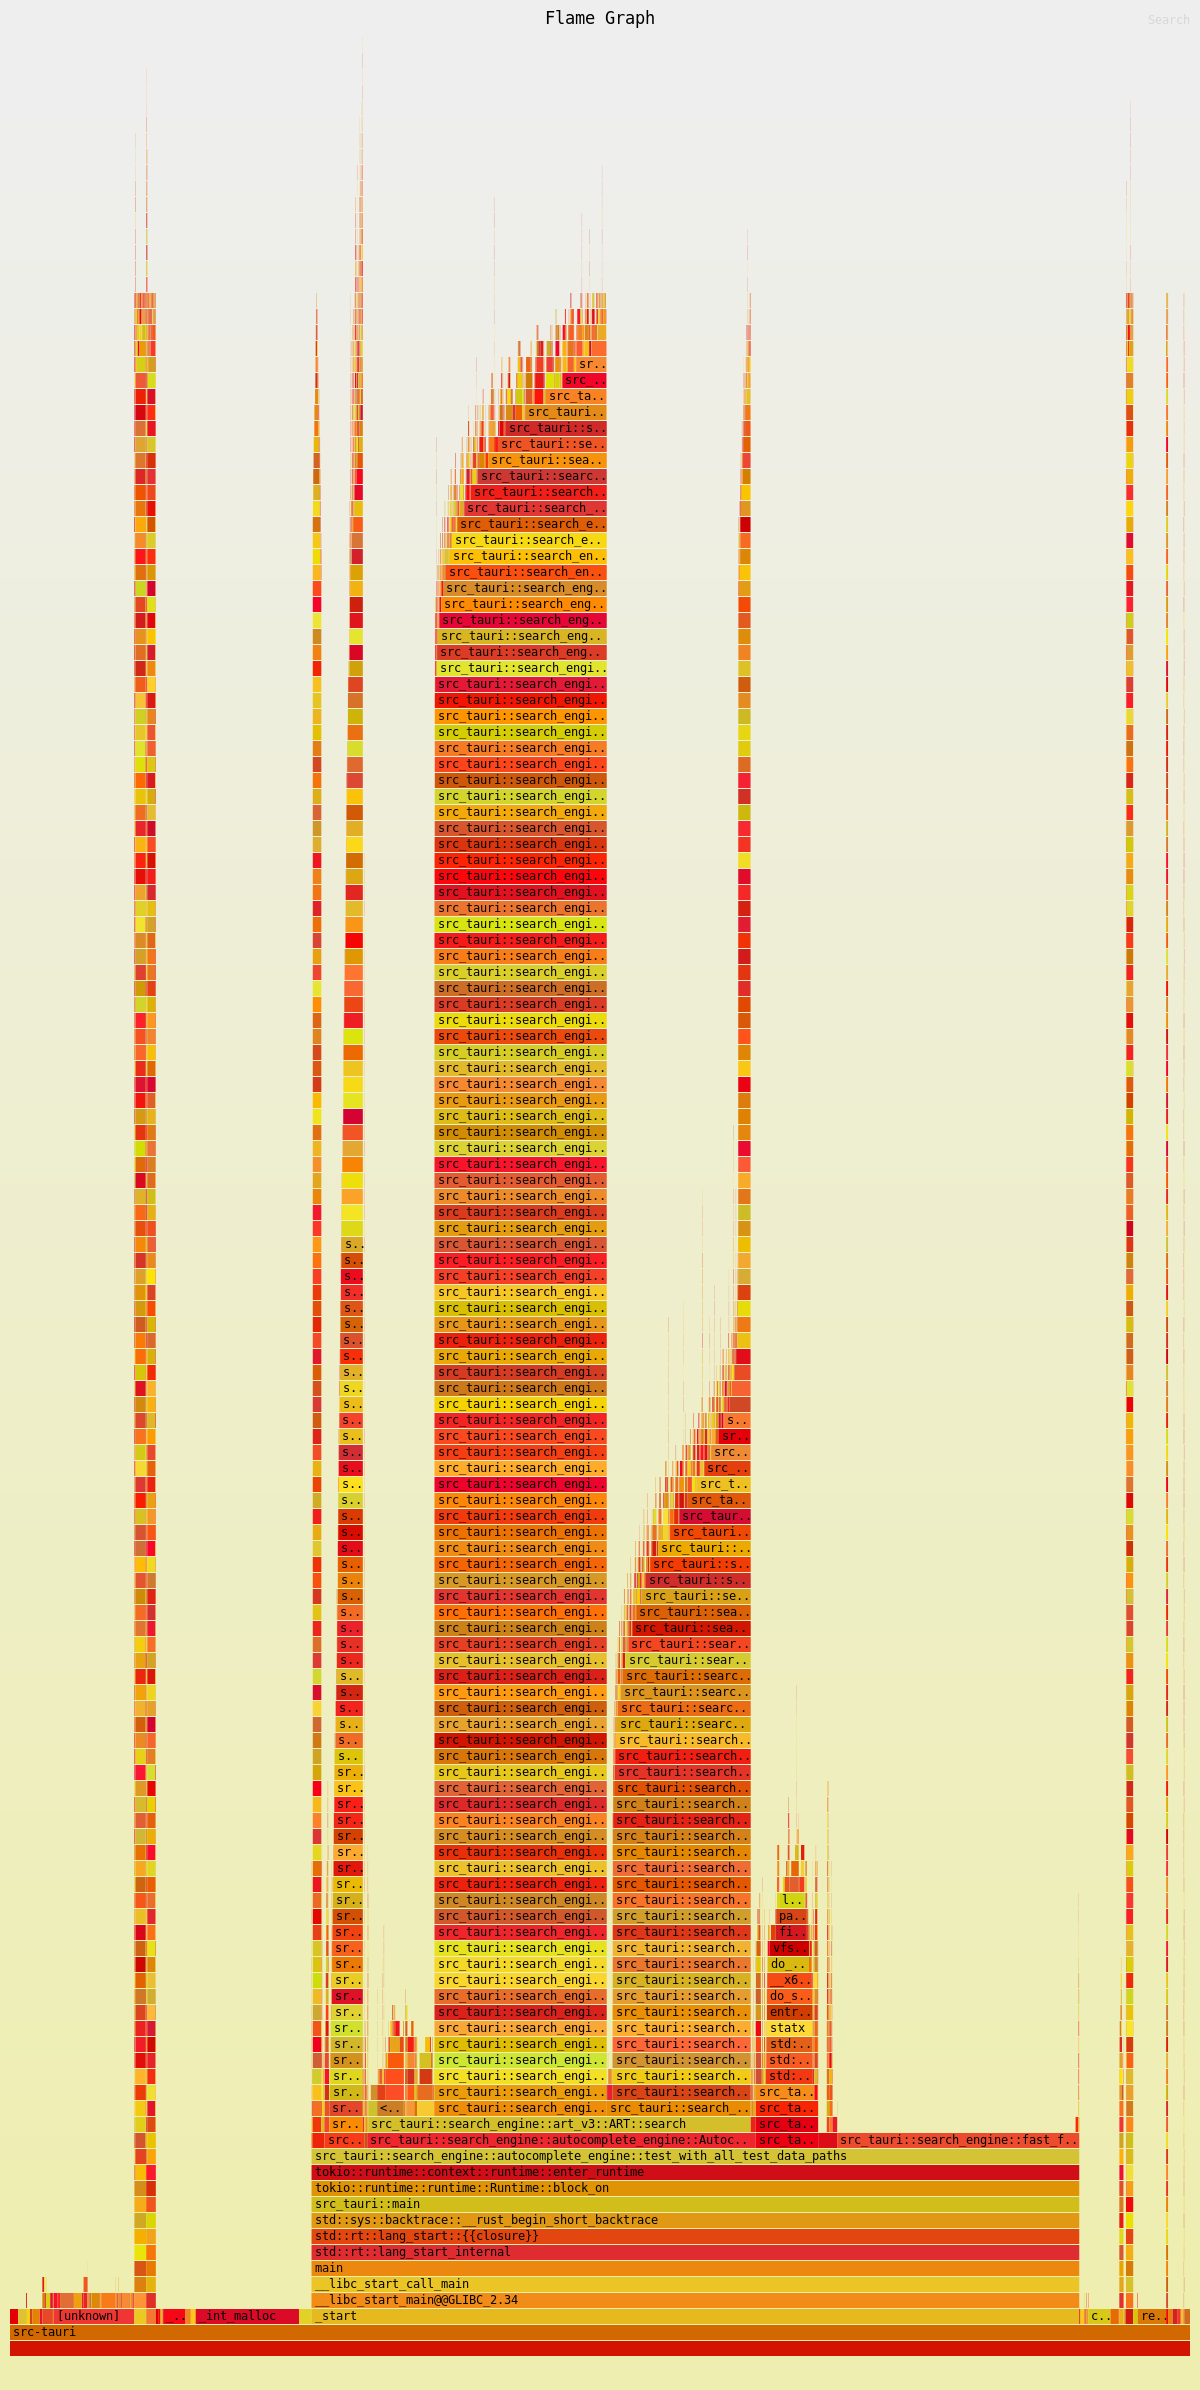
\includegraphics[width=0.7\textwidth]{./flamegraphs/test_with_all_test_paths.png}
  \caption{Flamegraph von einem Searchengine Durchlauf mit allen Einträgen der Testdaten}
  \label{fig:second_flame_graph}
\end{figure}

\begin{figure}[p]
  \centering
  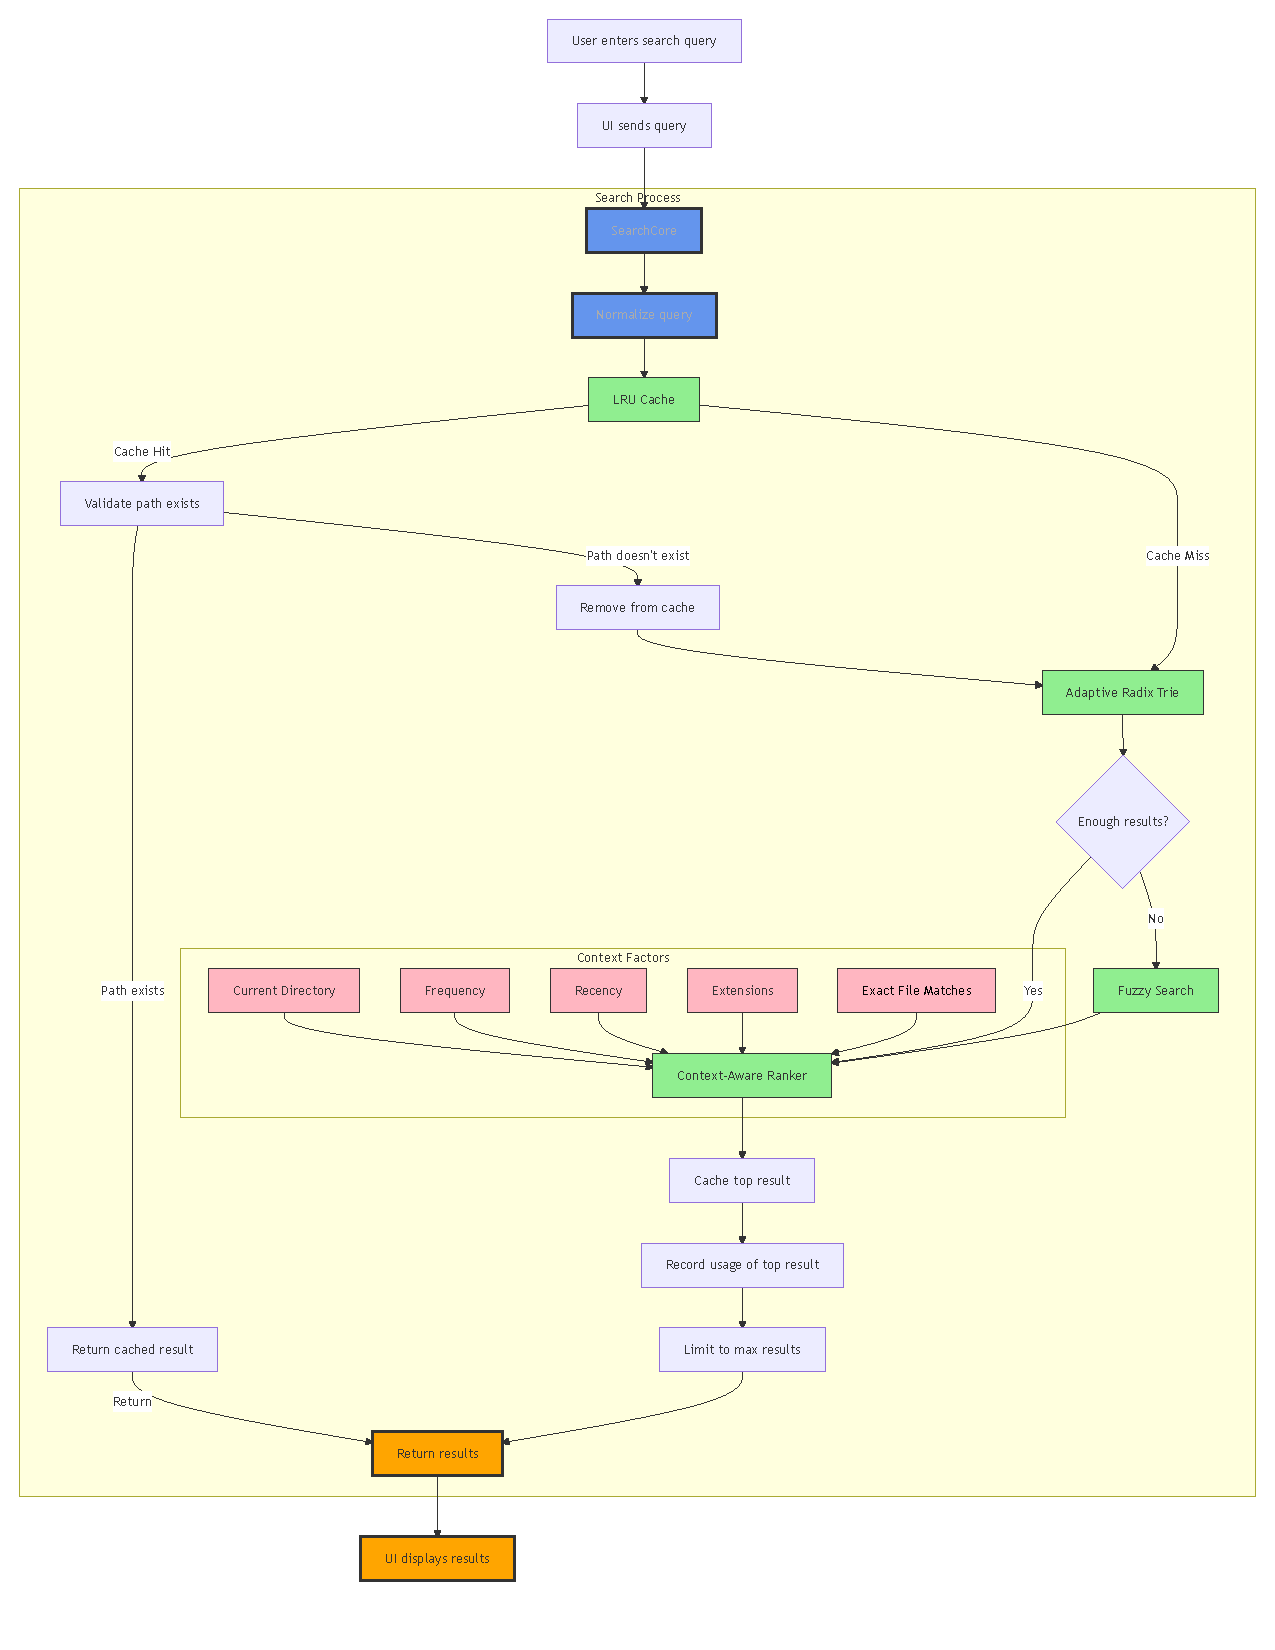
\includegraphics[width=0.9\textwidth]{./search_engine_images/diagram.pdf}
  \caption{Search engine Prozessdiagram}
  \label{fig:searchEngine}
\end{figure}

\begin{figure}[htbp]
  \centering
  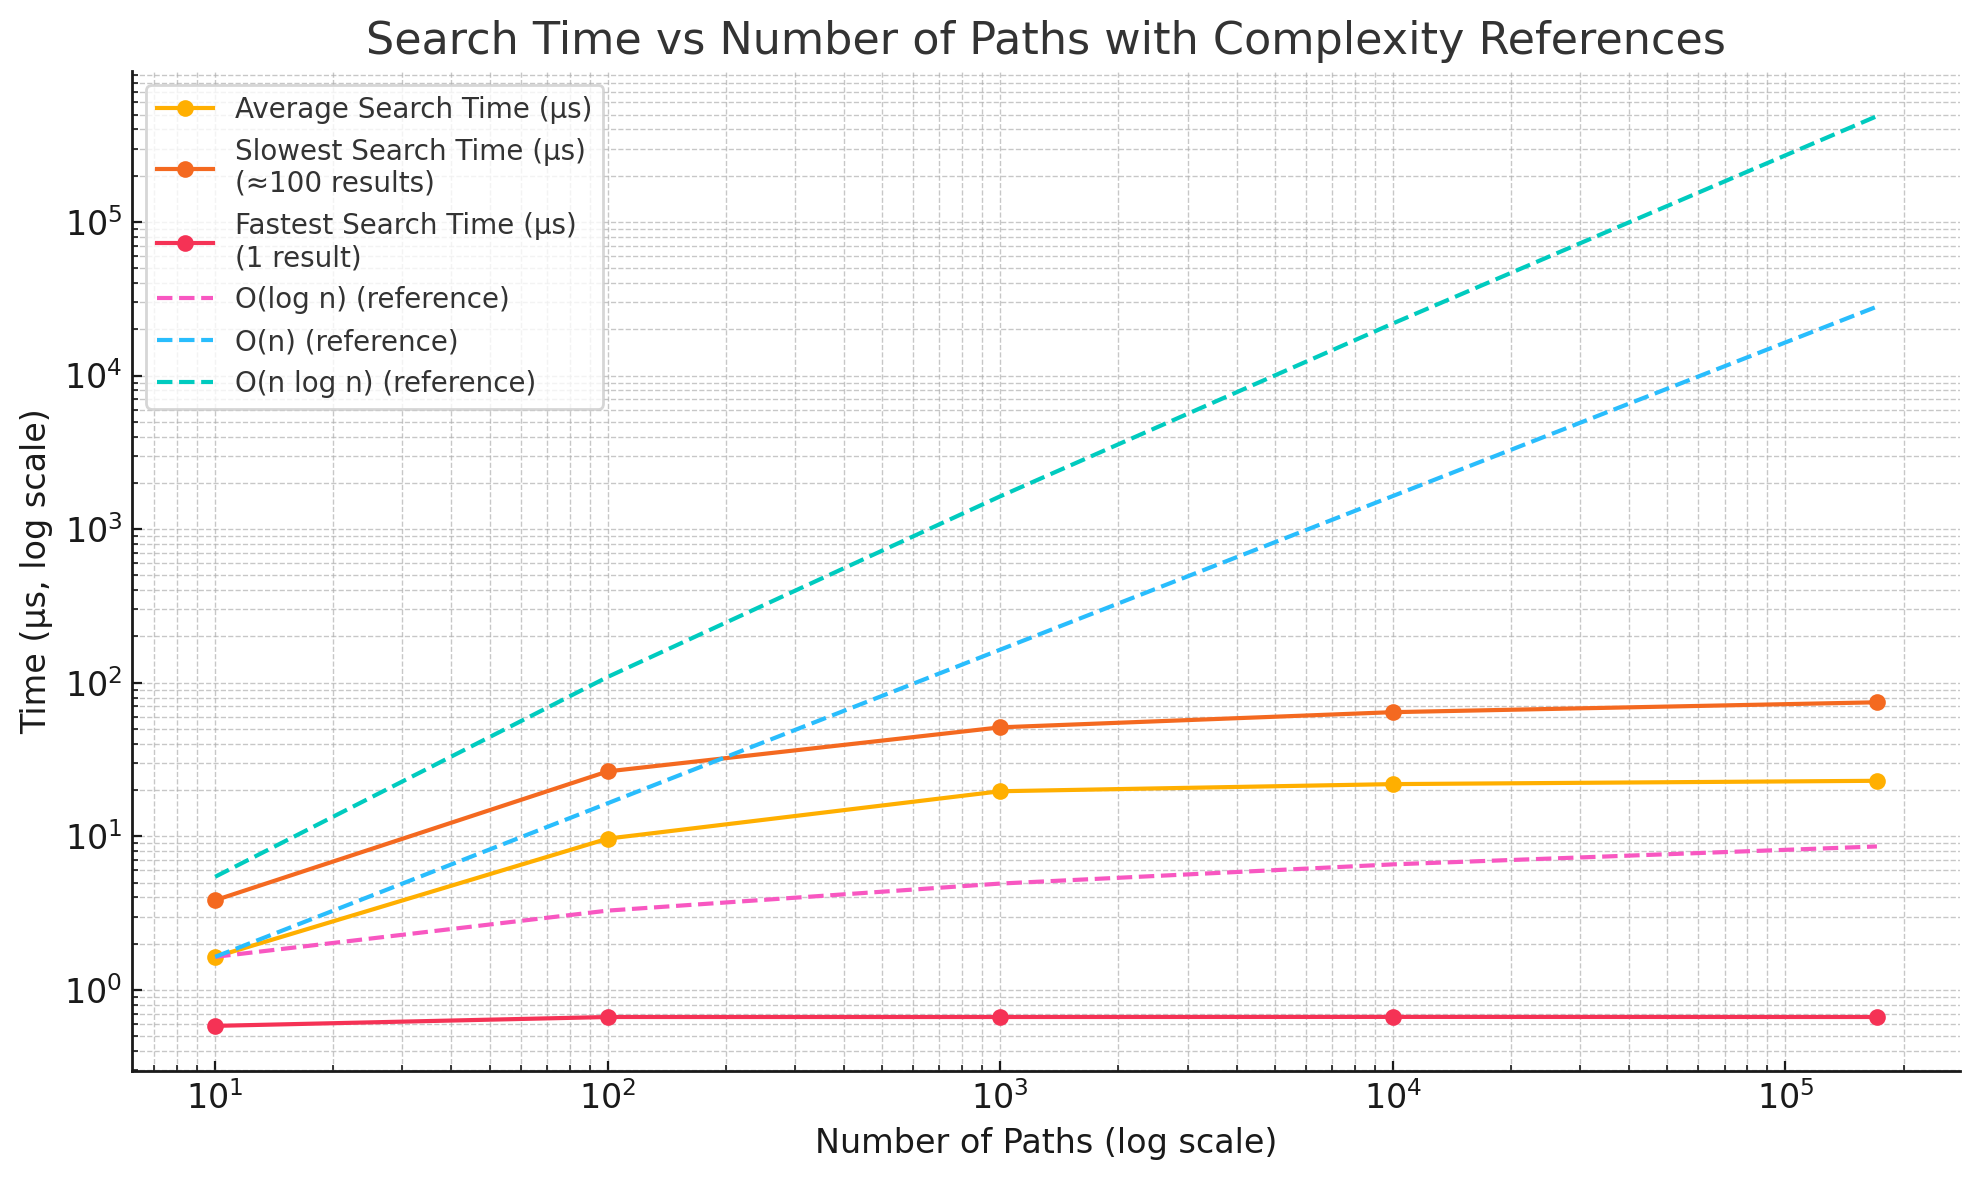
\includegraphics[width=0.7\textwidth]{./search_engine_images/art.png}
  \caption{Adaptive Radix Trie Zeitkomplexität}
  \label{fig:ART_time_complexity}
\end{figure}

\begin{figure}[htbp]
  \centering
  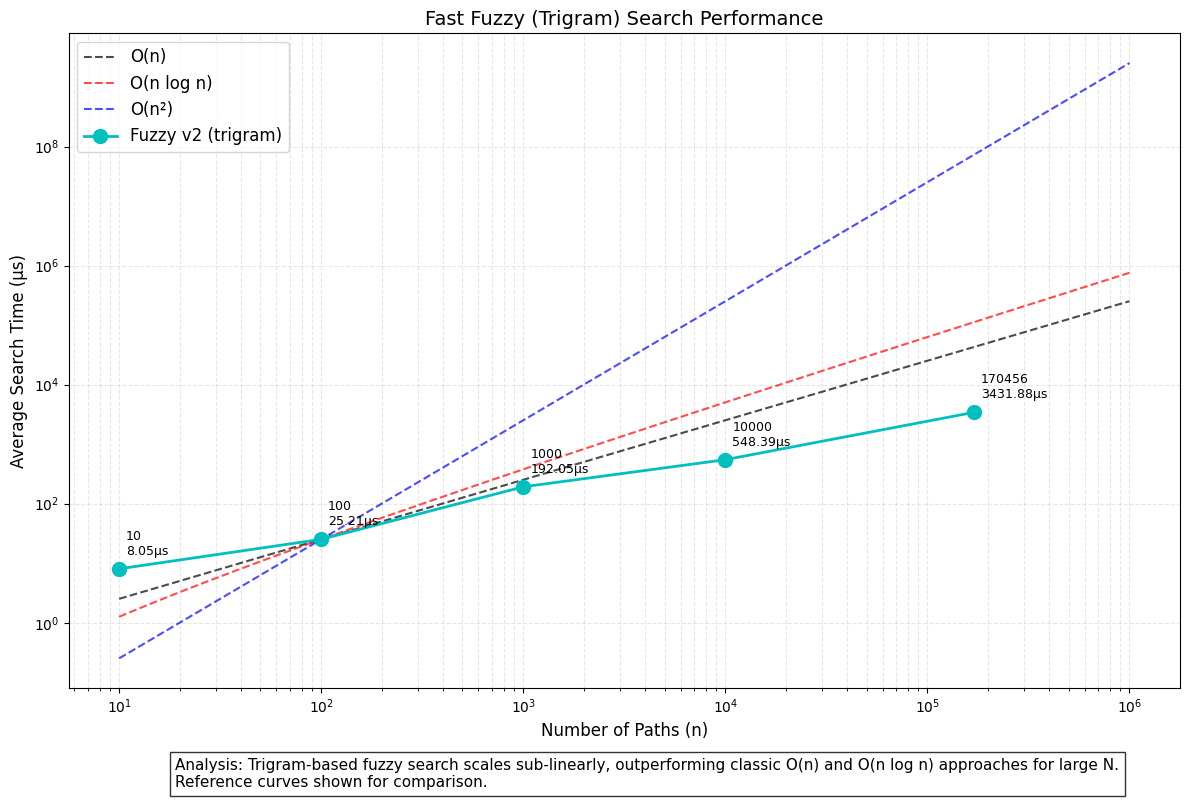
\includegraphics[width=0.7\textwidth]{./search_engine_images/fast_fuzzy.png}
  \caption{Fuzzy Suche Zeitkomplexität}
  \label{fig:fuzzy_time_complexity}
\end{figure}

\begin{figure}[htbp]
  \centering
  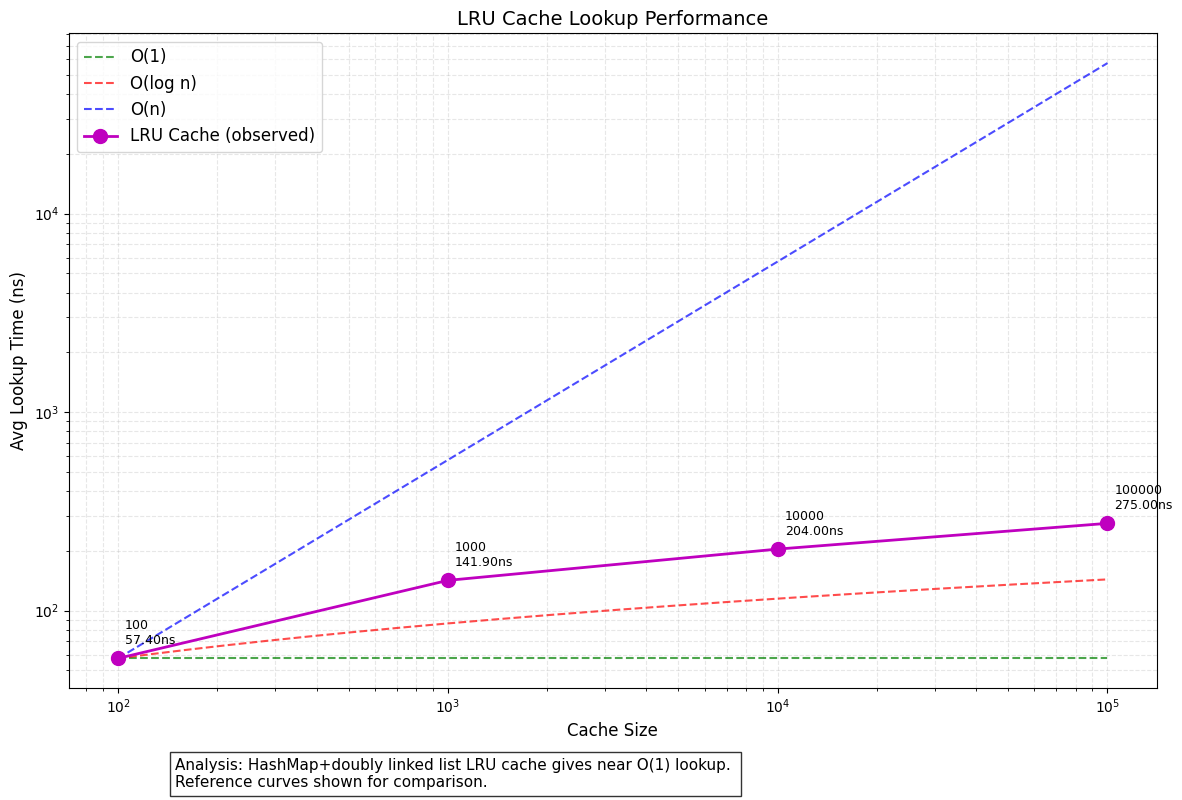
\includegraphics[width=0.7\textwidth]{./search_engine_images/lru_cache.png}
  \caption{LRU Cache Zeitkomplexität}
  \label{fig:lru_time_complexity}
\end{figure}
